\section{Conclusion}
\begin{frame}
\frametitle{How many users?}
\begin{columns}[c]
\column{0.5\textwidth}
\begin{block}{Hard to tell\ldots}
\begin{itemize}
    \item $\approx$ 600 members on the otb-users list
    \item Between 100 and 150 mails by months
    \item $\approx$ 100 members on the developers list
    \item $\approx$ 118 user accounts on the bug tracker
    \item $\approx$ 50 contributors in the documentation
    \item $\approx$ 3400 downloads for OTB 5.0 on SourceForge(released June 1, 2015).
  \end{itemize}
\end{block}
\begin{block}{2015, 2016 and 2017 Users Days}
  40 to 60 atendants in Toulouse during 3 days
\end{block}
\column{0.5\textwidth}
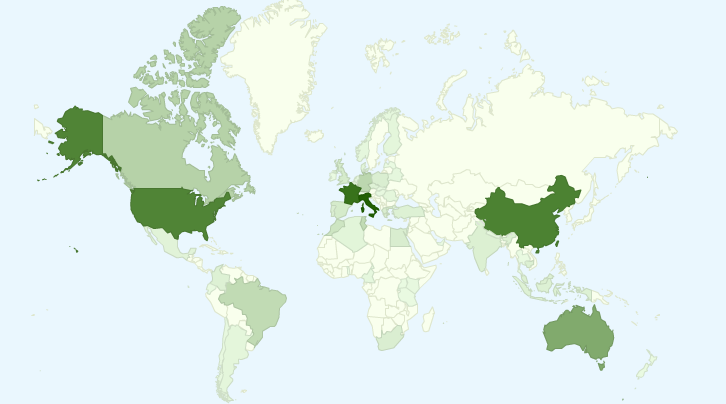
\includegraphics[width=0.9\textwidth]{images/OTB4_download_sourceforge_country_crop.png}\\
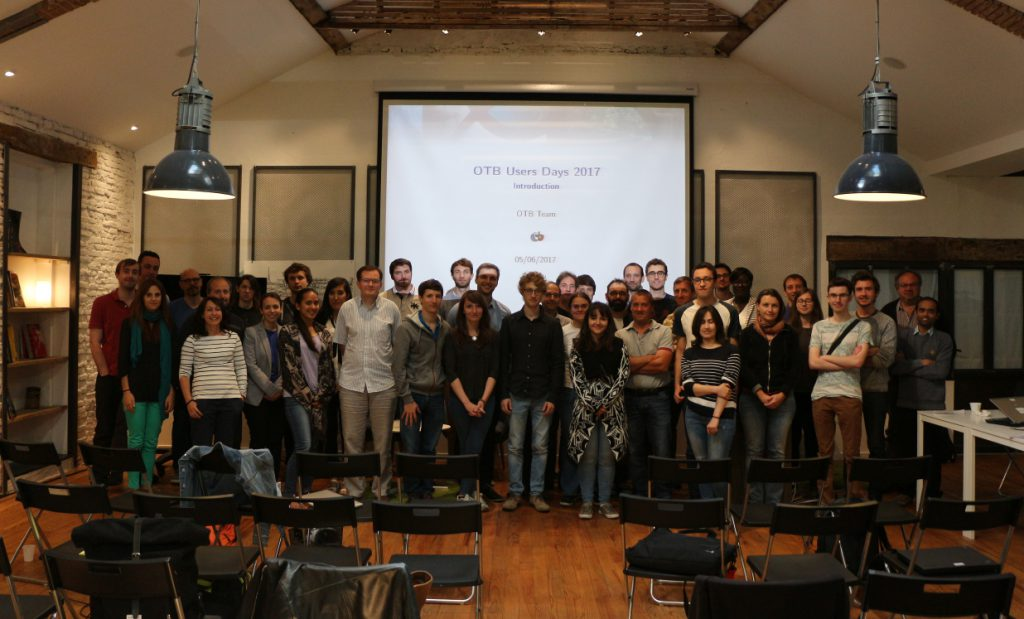
\includegraphics[width=0.9\textwidth]{images/userdays2017.jpg}
\end{columns}
\end{frame}

\begin{frame}
  \frametitle{Success stories}
  \vspace{-0.5cm}
\begin{columns}
\column{0.65\textwidth}
\begin{itemize}
\item OTB has been useful to ORFEO users and has processed 619 Pléiades
  images on RTU web site
\item Several training courses (3/5-day courses) given in France, Belgium,
Madagascar, UNESCO, Hawaii,Finland\ldots
\item OTB provides many useful RS functions in \textbf{one single tool}
\item OTB helped to improve the open-source codec for JP2 OpenJpeg
\item OTB equals or beats state-of-the-art tools (open source and maybe \$\$) on some points:
  \begin{itemize}
  \item band calculator
  \item tile-wise segmentation of full imagery
  \item full scene classification with a range of machine learning algorithms
  \item bridges between RS and GIS \ldots
  \end{itemize}
\item Beyond Orfeo, OTB is already used in several projects and software
\item OSGeo graduation
\end{itemize}
\column{0.35\textwidth}
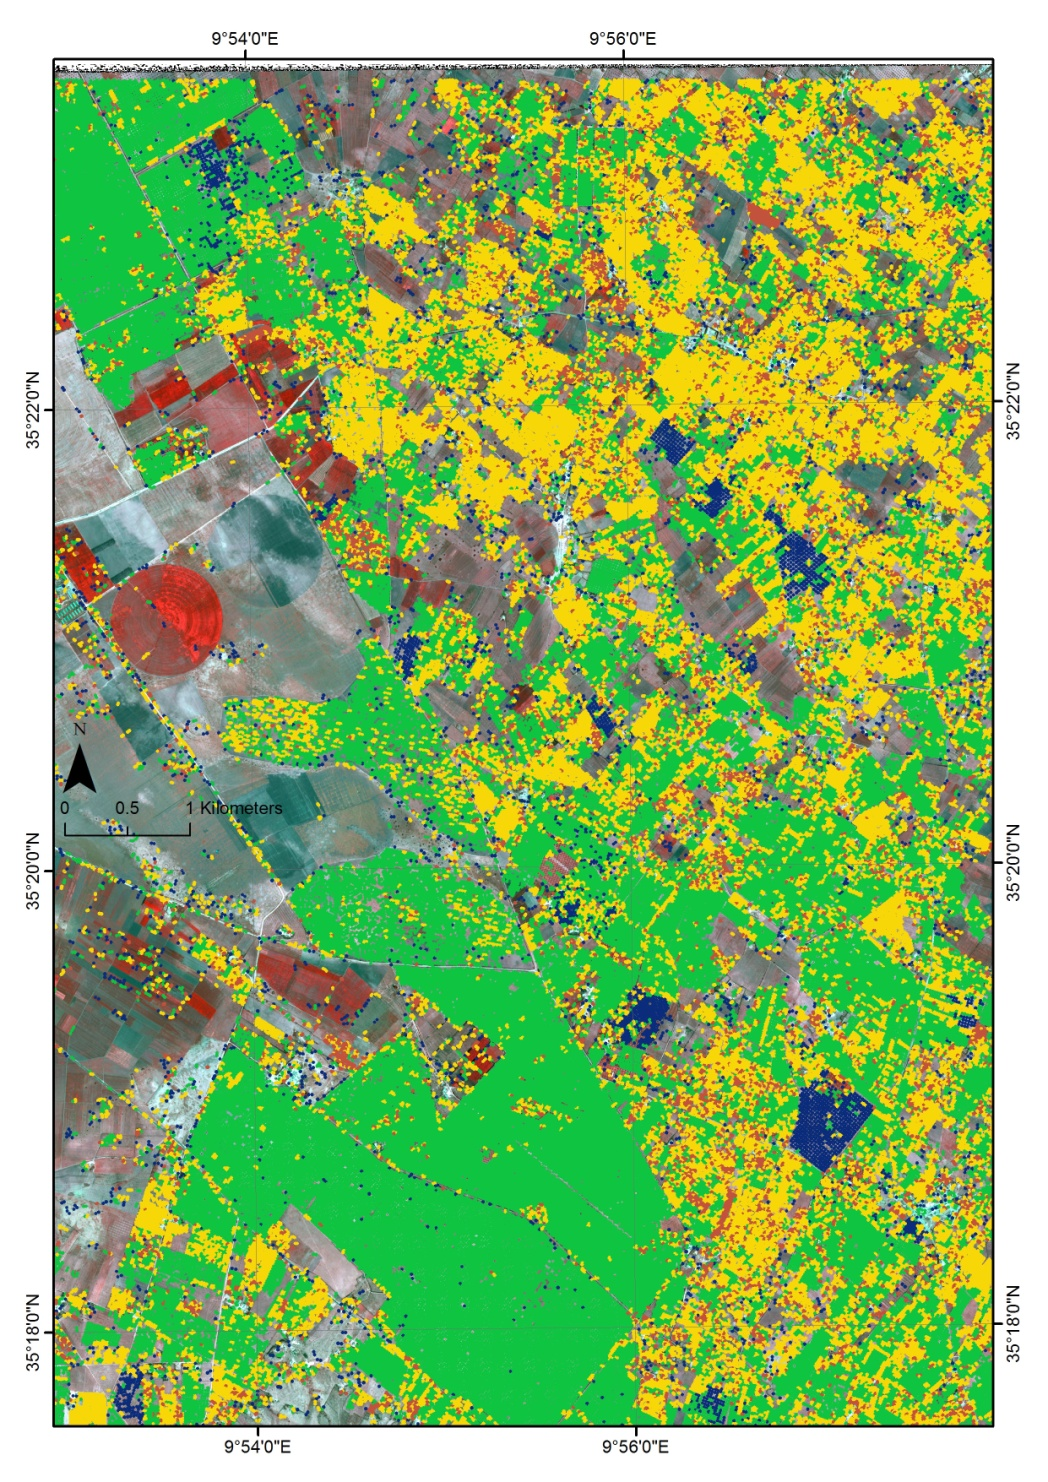
\includegraphics[width=0.9\textwidth]{images/resultats_ird.png}\\
\tiny{Thematic map from OTB segmentation, B. Mougenot~-~IRD}
\end{columns}
\end{frame}

\begin{frame}
  \frametitle{Projects and software using OTB}
  \vspace{-0.5cm}
\begin{columns}
  \column{0.55\textwidth}
  \begin{itemize}
    \item OTB applications are available in QGIS and in Zoo Project (WPS service)
    \item OTB is a component of \alert{Sentinel-2} and Venus ground segment (CNES and ESA)
    \item Terr'Image: Educational software for satellite image analysis
    \item Use to prototype \alert{THEIA} products from the Scientific Expertise Centres
    \item ESA Sentinel-2 for Agriculture
    \item Gnorasi Software (National Technical University of Athens)
    \item Geosud project(IRSTEA)
    \item TCM research program (ETS Quebec)
    \item Processing chains at CEREMA and SERTIT
  \end{itemize}
  \column{0.6\textwidth}
  \begin{center}
  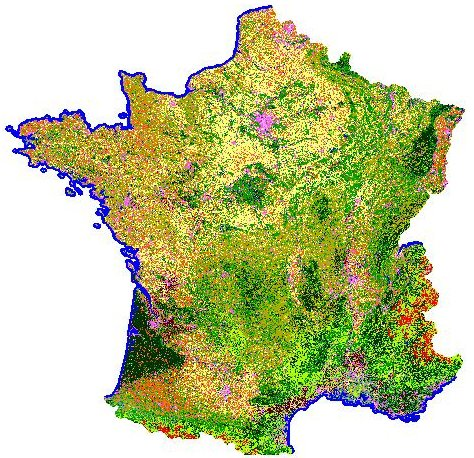
\includegraphics[width=0.6\textwidth,height=0.35\textheight]{images/oso-2017.jpeg}\\
  \tiny{Prototype of THEIA Land cover product (CESBIO)}
  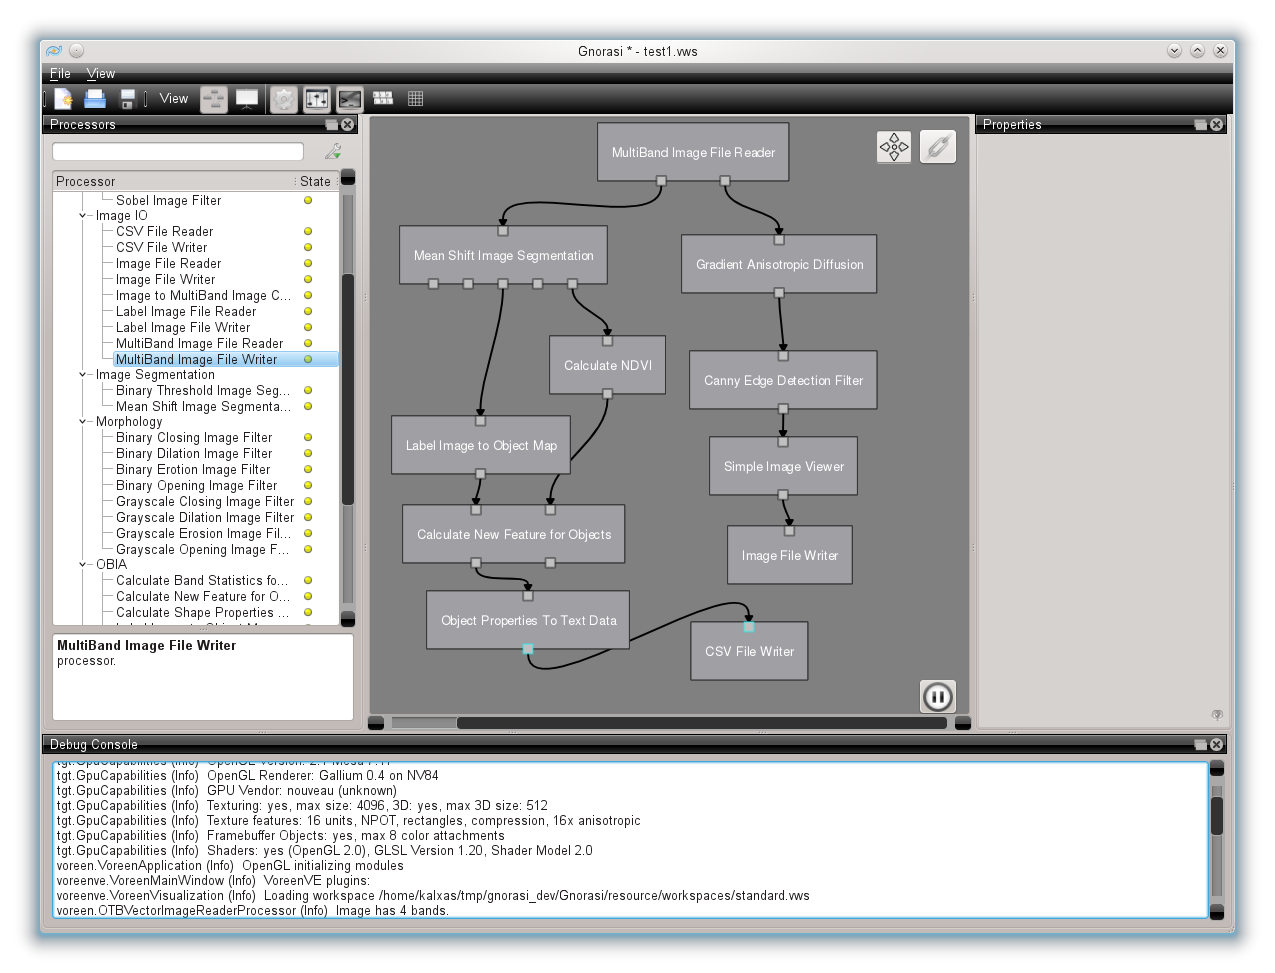
\includegraphics[width=0.6\textwidth,height=0.35\textheight]{images/gnorasi2.png}\\
  \tiny{The Gnorasi software}
  \end{center}
\end{columns}
\end{frame}

\begin{frame}
\frametitle{Support/Help/Contribute}
\vspace{-0.2cm}
\begin{block}{General resources}
\vspace{-0.2cm}
\begin{description}
\item[Site web] \href{http://www.orfeo-toolbox.org}{orfeo-toolbox.org}
\item[Wiki] \href{http://wiki.orfeo-toolbox.org}{wiki.orfeo-toolbox.org}
\item[Blog] \href{http://blog.orfeo-toolbox.org}{blog.orfeo-toolbox.org}
\end{description}
\end{block}
\vspace{-0.2cm}
\begin{block}{Documentation and help}
\vspace{-0.2cm}
\begin{description}
\item[Guides] Software Guide and CookBook (remote sensing recipes)
\item[Doxygen] \href{http://www.orfeo-toolbox.org/doxygen}{doxygen}
\item[Users mailing list] otb-users@googlegroups.com
\item[Developers mailing list] otb-developers@googlegroups.com
\end{description}
\end{block}
\vspace{-0.2cm}
\begin{block}{Follow-up}
\vspace{-0.2cm}
\begin{description}
\item[Look at the code?] \href{https://gitlab.orfeo-toolbox.org/orfeotoolbox/otb}{gitlab.orfeo-toolbox.org}
\item[Find a bug? Feature propositions?] \href{https://gitlab.orfeo-toolbox.org/orfeotoolbox/otb/issues}{gitlab.orfeo-toolbox.org/orfeotoolbox/otb/issues}
\item[Dashboard] \href{http://dash.orfeo-toolbox.org}{dash.orfeo-toolbox.org}
\end{description}
\end{block}
\end{frame}

\begin{frame}
\frametitle{Thank you! Any questions?}
\begin{minipage}[t][6cm][t]{\textwidth}
\begin{center}
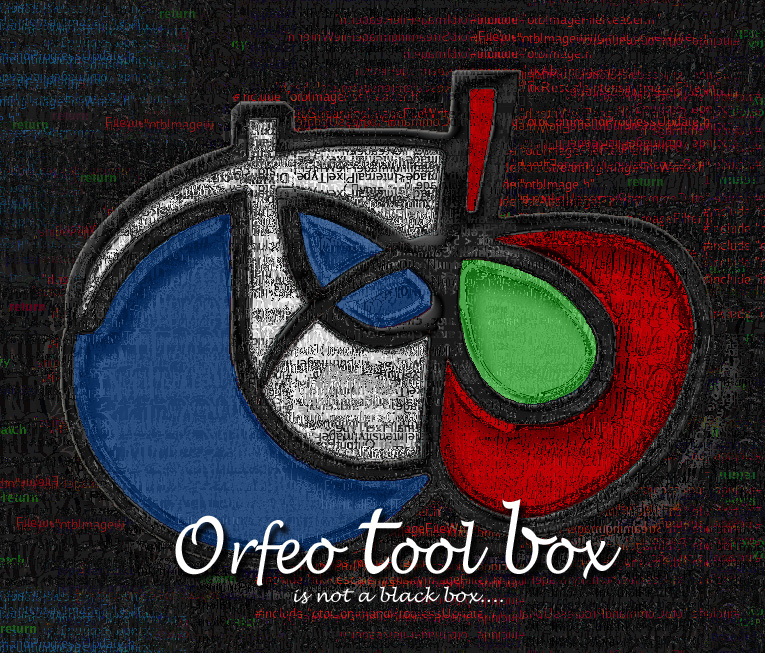
\includegraphics[width=0.65\textwidth]{images/LOGOTB_blackbox.png}
\end{center}
\end{minipage}
\end{frame}
